% Part: sets-functions-relations
% Chapter: relations
% Section: trees

\documentclass[../../../include/open-logic-section]{subfiles}

\begin{document}

\olfileid{sfr}{rel}{tre}
\olsection{वृक्ष}

तर्कशास्त्राच्या सर्व शाखांत महत्त्वाची भूमिका बजावणारा अंशतः क्रमाचा
एक विशिष्ट प्रकार म्हणजे \emph{वृक्ष}. तर्कशास्त्राच्या प्राथमिक भागांत
सांत वृक्ष येतात: उदाहरणार्थ, !!{formula}s विन्यासवृक्षात विभागून
समजून घेता येतात, आणि अनेक !!{derivation} पद्धतींतील
!!{derivation}s सुद्धा सांत वृक्षांच्या स्वरूपात असतात.
%
विधानीय आणि प्रथमस्तरीय तर्कशास्त्राच्या परिपूर्णता प्रमेयांच्या सिद्धतेतच
अनंत वृक्ष येऊ लागतात; पुढे संपूर्ण गणिती तर्कशास्त्रात त्यांचा वापर होतो.

वृक्षाची संचसैद्धान्तिक संकल्पना आणि आलेख सिद्धांतातील वृक्षाची संकल्पना
यांचा निकटचा संबंध आहे. एका सांत वृक्षाचे चित्र असे आहे:

\begin{center}
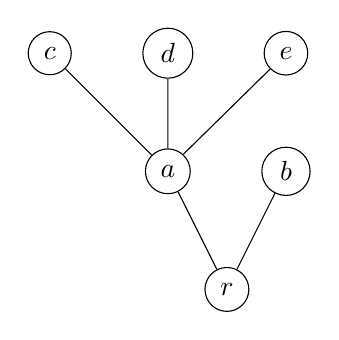
\begin{tikzpicture}[nodes={draw, circle}, -]
\node{$r$} [grow'=up]
    child { node {$a$}
        child { node {$c$} }
        child { node {$d$} }
        child { node {$e$} }
    }
    child { node {$b$} };
\end{tikzpicture}
\end{center}

सर्वांत खालचे $r$ हे शिखर मूळ आहे. $r$ व्यतिरिक्त प्रत्येक शिखराच्या
लगेच खाली नेमके एक पालक शिखर आहे. $x$ पासून कडांवरून वर जात $y$ पर्यंत
पोहोचता येत असेल, तर $x$ चा $y$ शी असणारा संबंध म्हणजे $x$ हा $y$ चा
\emph{पूर्वज} असणे, असे समजू शकतो.

वृक्षातील पूर्वज संबंध हा काटेकोर अंशतः क्रम असतो. यावरून संचसैद्धान्तिक
व्याख्या सुचते. ती मांडण्यासाठी दोन संकल्पना लागतात. $\le$ ने अंशतः
क्रमित केलेल्या $A$ या संचातील \emph{लघुतम घटक} म्हणजे असा
!!a{element} $x \in A$ की सर्व $y \in A$ साठी $x \le y$ असते.
एखाद्या संचाच्या प्रत्येक अरिक्त उपसंचात लघुतम घटक असेल, तर तो संच
$\le$ ने \emph{सुक्रमित} आहे असे म्हणतात.

\begin{defn}[वृक्ष]
\emph{वृक्ष} म्हणजे $T = \tuple{A, \le}$ अशी जोडी की $A$ हा संच असतो,
$\le$ हा $A$ वरील अंशतः क्रम असतो, त्याचा $r \in A$ हा एकमेव लघुतम
घटक असतो (त्याला \emph{मूळ} म्हणतात), आणि सर्व $x \in A$ साठी
$\Setabs{y}{y \le x}$ हा संच $\le$ ने सुक्रमित असतो.
\end{defn}

\begin{defn}[उत्तरवर्ती]
$T = \tuple{A, \le}$ हा वृक्ष आहे असे समजा.
$x,y \in A$, $x < y$ असतील आणि $x < z < y$ असा कोणताही $z \in A$
नसेल, तर $y$ हा $x$ चा \emph{उत्तरवर्ती} आहे असे म्हणतो.
\end{defn}

$x \in A$ च्या उत्तरवर्तींना त्याची \emph{अपत्ये} असेही म्हणतात.
$y$ हा $x$ चा उत्तरवर्ती असेल, तर $x$ ला $y$ चा \emph{पूर्ववर्ती}
किंवा \emph{पालक} म्हणतो.

\begin{prop}
$\tuple{A,\le}$ हा वृक्ष असेल, तर मूळ वगळता प्रत्येक $x \in A$ ला
जास्तीत जास्त एक पूर्ववर्ती असतो.
\end{prop}

\begin{proof}
  $y_1 < x$, $y_2 < x$ आणि $y_1 \neq y_2$ असे समजा. मग
  $\{y_1, y_2\} \subseteq \Setabs{z}{z<x}$. $\Setabs{z}{z<x}$ हा संच
  $\le$ ने सुक्रमित असल्याने त्याच्या $\{y_1, y_2\}$ या उपसंचाला लघुतम
  घटक असतो. तो स्पष्टपणे $y_1$ किंवा $y_2$ असला पाहिजे. म्हणून
  $y_1 \le y_2$ किंवा $y_2 \le y_1$. आपण $y_1 \neq y_2$ गृहीत धरले,
  म्हणून प्रत्यक्षात $y_1 < y_2$ किंवा $y_2 < y_1$. शिवाय,
  $y_1 < x$ आणि $y_2 < x$ या गृहीतकांमुळे $y_1 < y_2 < x$ किंवा
  $y_2 < y_1 < x$. म्हणून $y_1$ आणि $y_2$ हे दोघेही $x$ चे पूर्ववर्ती
  असू शकत नाहीत.
\end{proof}

\begin{defn}
$T = \tuple{A, \le}$ या वृक्षातील $A$ हा अनंत संच असेल, तर वृक्षाला
\emph{अनंत}, आणि अन्यथा \emph{सांत} म्हणतात. $T$ मधील प्रत्येक
$x \in A$ ला फक्त सांत संख्येने उत्तरवर्ती असतील, तर $T$ ला
\emph{सांत शाखनाचा} वृक्ष म्हणतात.
\end{defn}

\begin{defn}[शाखा]
$T = \tuple{A, \le}$ हा वृक्ष दिला असता, $T$ ची \emph{शाखा} म्हणजे
$T$ मधील अधिकतम शृंखला; म्हणजे $B \subseteq A$ असा संच की कोणत्याही
$x, y \in B$ साठी $x \le y$ किंवा $y \le x$ असते, आणि प्रत्येक
$z \in X \setminus B$ साठी असा $u \in B$ असतो की $z \le u$ आणि
$u \le z$ दोन्ही असत्य असतात.
%
$T$ च्या सर्व शाखांचा संच दर्शवण्यासाठी आपण $[T]$ वापरतो.
\end{defn}

\begin{ex}
सांत शाखनाच्या वृक्षाचे एक प्रसिद्ध उदाहरण म्हणजे $0$ आणि $1$ यांच्या
सांत अनुक्रमांचा \emph{अनंत द्विमान वृक्ष}. त्याला कधी $\{0,1\}^*$ किंवा
$\Bin^*$ असे लिहितात आणि विस्तार संबंध $\sqsubseteq$ ने क्रमित करतात
(उदा., $101 \sqsubseteq 101101$). कोणत्याही द्विमान चिन्हमालेच्या शेवटी
$0$ किंवा $1$ जोडून तिचा विस्तार नेहमी करता येतो. म्हणून या वृक्षात
अनंत घटक असतात: प्रत्येक $s$ या घटकाला नेमके दोन उत्तरवर्ती, $s0$ आणि
$s1$, असतात. त्याचे मूळ म्हणजे $\emptyseq$ हा रिक्त अनुक्रम.
\end{ex}

\begin{ex}
थोडे अधिक सर्वसाधारण उदाहरण म्हणजे नैसर्गिक संख्यांच्या सांत अनुक्रमांचा
$\Nat^*$ हा संच आणि त्यावरील विस्तार संबंध $\sqsubseteq$; हाही वृक्ष
असतो. तो स्पष्टपणे सांत शाखनाचा नाही: प्रत्येक $s \in \Nat^*$ ला अनंत
उत्तरवर्ती $sn$ असतात, प्रत्येक $n \in \Nat$ साठी एक. $\sqsubseteq$
नुसार बंद असलेला प्रत्येक $A \subseteq \Nat^*$ हा $\Nat^*$ चा
\emph{उपवृक्ष} असतो. (म्हणजे $A$ असा आहे की $s \in A$ आणि
$s' \sqsubseteq s$ असतील, तर $s' \in A$ सुद्धा.) सर्व सांत वृक्ष
$\Nat^*$ चे सांत उपवृक्ष म्हणून दर्शवता येतात.
\end{ex}

\begin{prop}[K\H{o}nig यांचे उपप्रमेय]
$T = \tuple{A,\le}$ हा सांत शाखनाचा अनंत वृक्ष असेल, तर $T$ ला
एक अनंत शाखा असते.
\end{prop}

संगणनीयता सिद्धांतात वारंवार वापरले जाणारे K\H{o}nig यांच्या उपप्रमेयाचे
एक विशेष रूप, ज्याला \emph{दुर्बल K\H{o}nig उपप्रमेय} म्हणतात, असे आहे:
$\{0,1\}^*$ च्या प्रत्येक अनंत उपवृक्षाला एक अनंत शाखा असते.

\end{document}
